\ifdefined\included
\else
\setcounter{chapter}{4} %% Numéro du chapitre précédent ;)
\dominitoc
\faketableofcontents
\fi

\chapter{Ontology-based Referring Expression Generation}
\chaptermark{Ontology-based REG}
\label{chap:4}
\minitoc

The contribution presented in this chapter is excerpted from our work, published in the proceedings of the RO-MAN 2020 conference~\cite{buisan_2020_efficient}. In this manuscript, the contribution is more detailed and discussed. The presented work has been achieved in collaboration with Guilhem Buisan, with an equal contribution. Several algorithms have been developed by both of us, giving, as a result, the one presented in this chapter, merging the best of our trials. My focus was mainly on how to fully take advantage of the ontology as a knowledge base and on algorithmic optimisations to make our method the most efficient in the current literature.

\section{Introduction}

Referring to an entity is one of the most common task that we perform every day. ``Can you bring me my mug? It is the black one next to the sink''. ``I don't remember the name of the man with the red shirt and the glasses''. ``I lost my keys, they are on a keychain with a unicorn-shaped plush toy''. Such kind of communication, precise and efficient, is a key apect for the success of a collaborative task. Nevertheless, in complex environment with a wide variety of objects, places, or people, referring a specific entity can become a real challenge for robotic application. The robot has to take into account the context of the upper task, the diversity of facts that can be extracted from the situation and which depend on available perception modalities, and the available common ground between the robot and its partner. 

\begin{figure}[ht!]
\centering
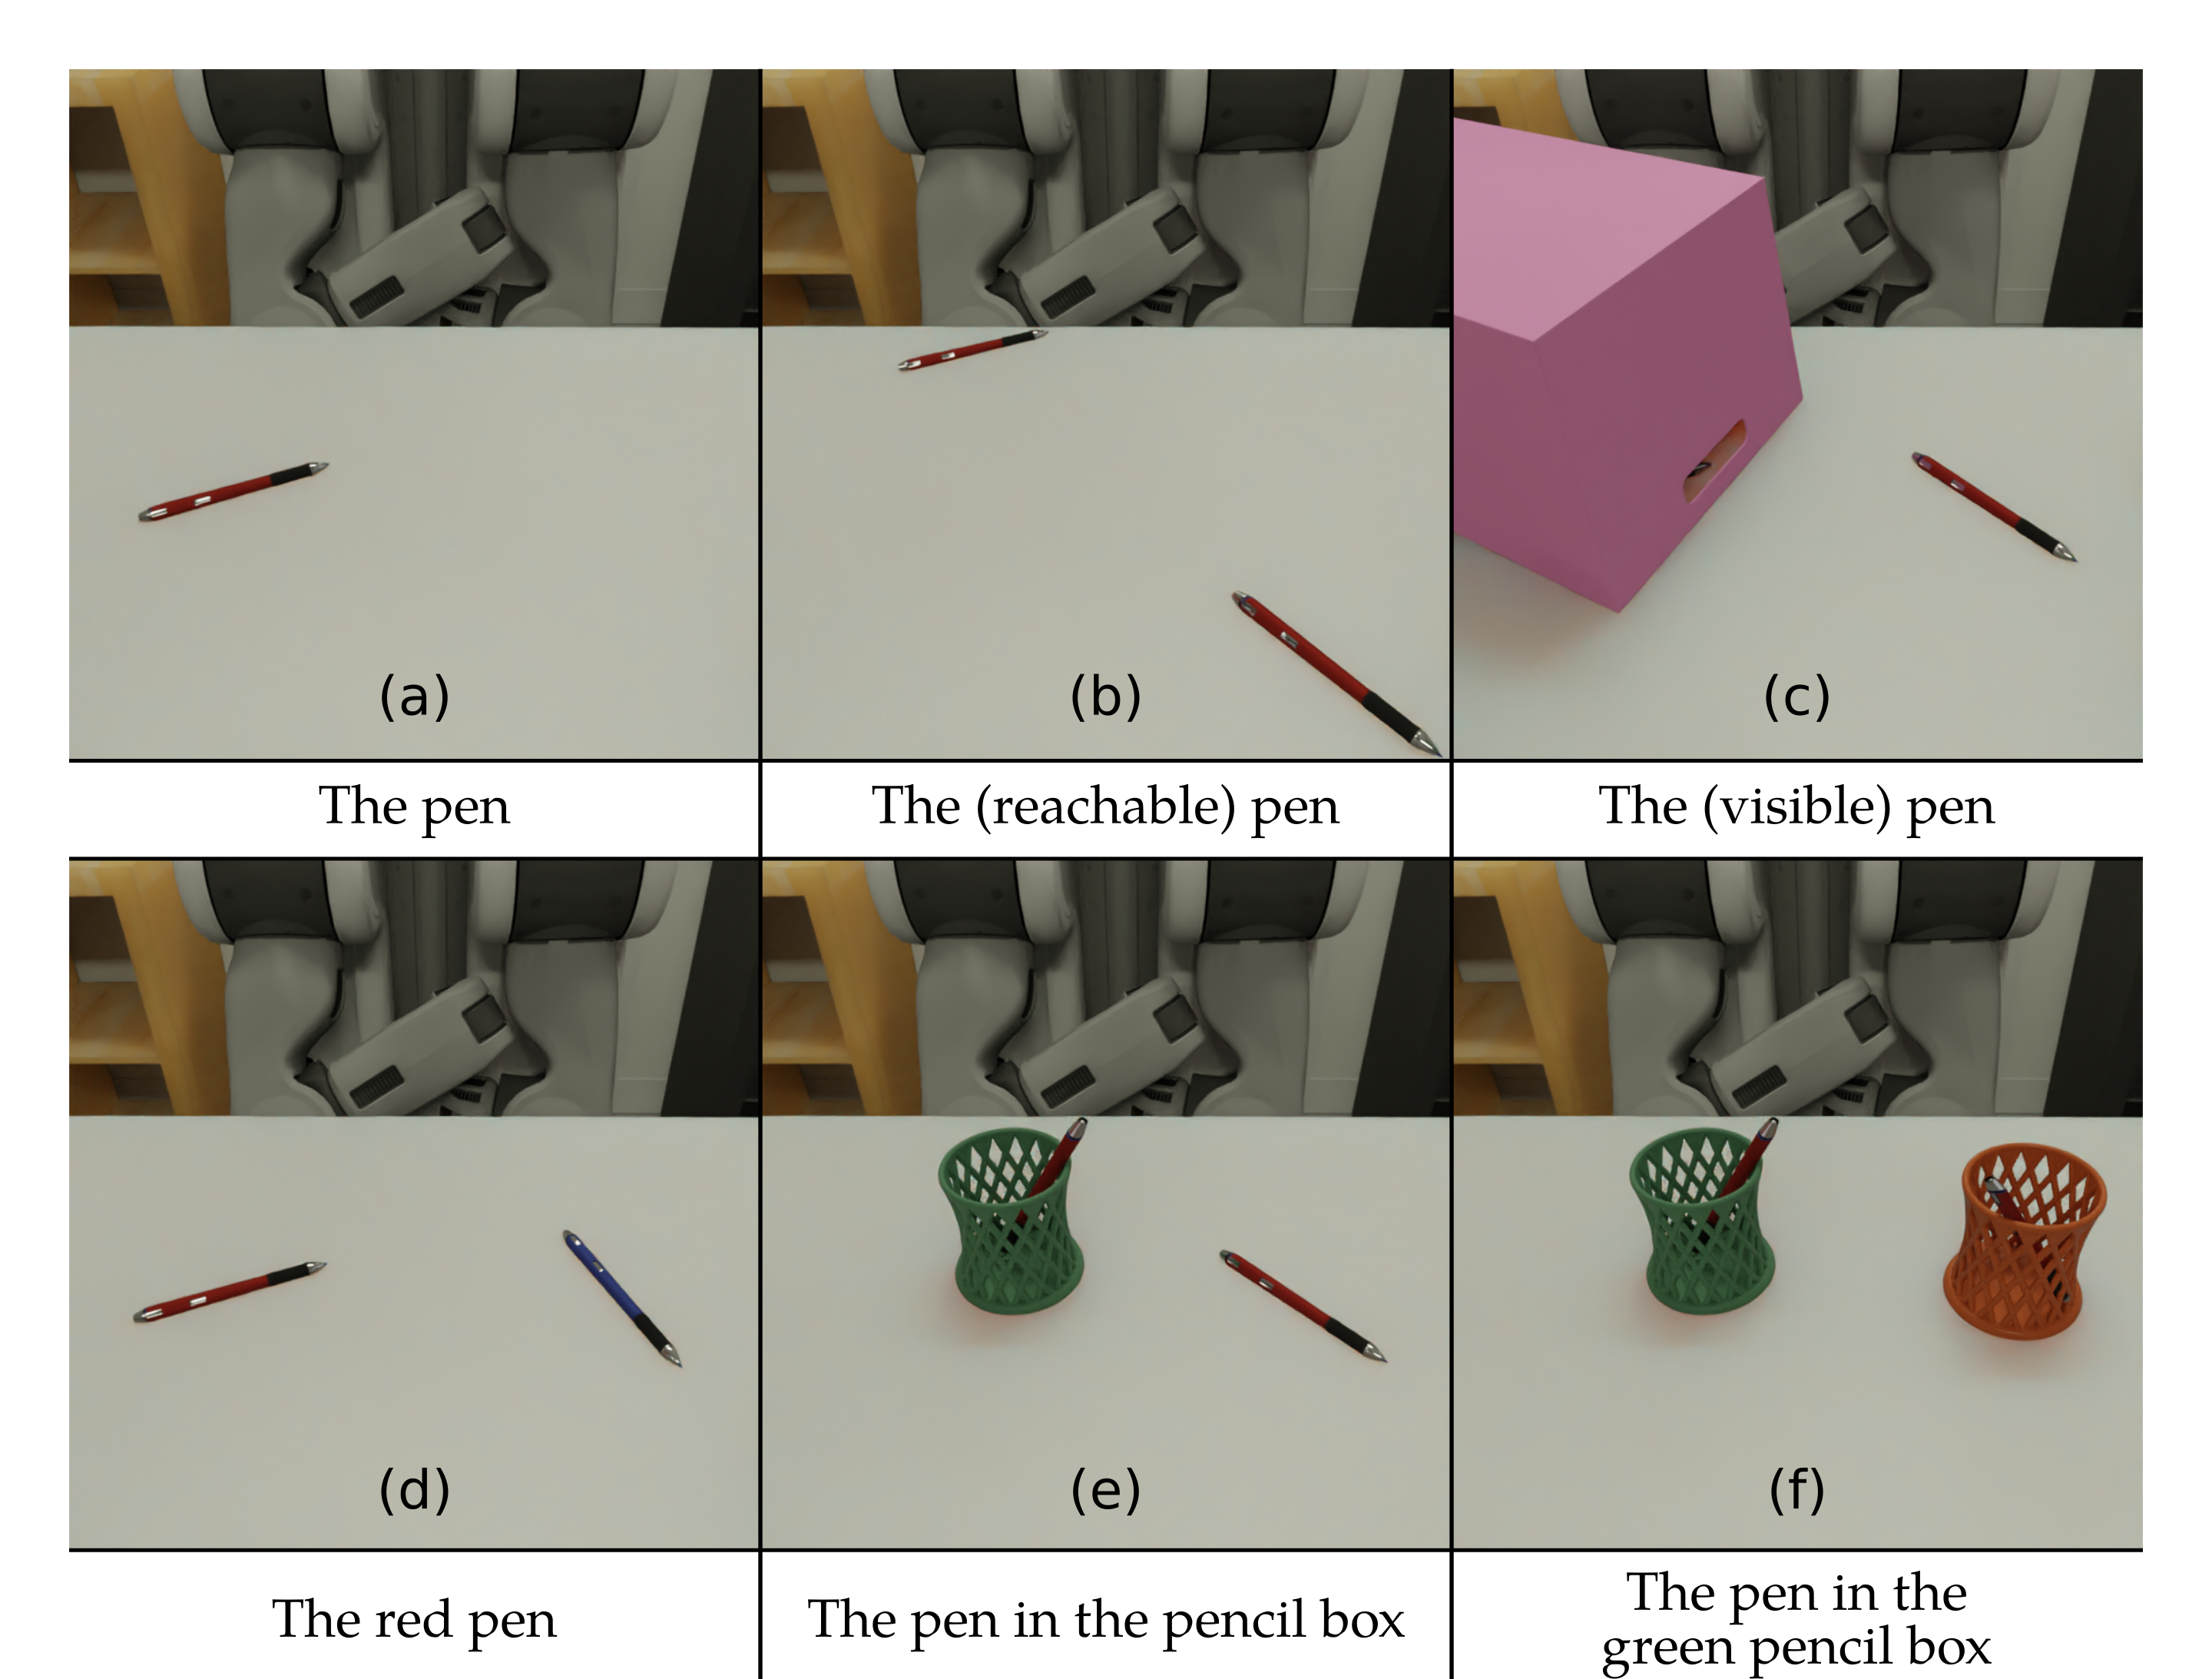
\includegraphics[scale=0.16]{figures/chapter4/intro.png}
\caption{\label{fig:chap4_intro} Six situations view from the hearer perspective, with the robot placed on the other side of the table. Referring to the same pen involves different mechanisms to raise the ambiguity, in each situation. The sentence above each situation is a possible referring expression to refer to said pen unambiguously. }
\end{figure}

Consider the situation where you are around a table with your collaborative robot and the robot needs a pen. The simple statement \textit{``Give me the pen''} can result in several situations of different complexities. In the case where there is only one pen (Fig.\ref{fig:chap4_intro}a), referring to it is obvious. Now consider two pens on the table. If one is reachable by you (the human) and the other is not (Fig.\ref{fig:chap4_intro}b), reachability can be used to refer to the pen. If both pens are not reachable but one is visible to you and the other is not (Fig.\ref{fig:chap4_intro}c where a pen is hidden under the box), visibility through perspective-taking could be used to determine that the other pen does not lead to ambiguity. Now both pens are visible and reachable, but one is blue and the other is red (Fig.\ref{fig:chap4_intro}d). The addition of the color of the pen solves the ambiguity. If both pens have the same color but one is in a pencil box (Fig.\ref{fig:chap4_intro}e), the relation to the pencil box resolves the ambiguity. If unfortunately, both are in a pencil box but one is green and the other orange (Fig.\ref{fig:chap4_intro}f), the relation to the pencil box and the color of the latter resolves the ambiguity. We could continue like this for a long time, considering that one is at your left and one at your right, that there is no pen on the table but there is one on a shelf and so on.

Until now, we considered that the robot knows the concepts of pen and pencil box as well as their names in natural language to speak about them. However, imagine yourself travelling in another country and having to speak english\footnote{I apologize to the native English speakers who will not take full advantage of this example.}, you can sometimes miss some words and thus use more generic a one instead. However, by doing so some new ambiguity can be raised because this generic word also refers to other entities. It is the same for our robot if it has to speak French and does not know the translation of the pencil box concept. It will have to use to a more generic term, such as ``container'' that can also refer to a box beside.

\improvement{ensure that ToM is defined before}
In addition to the concepts names, the robot must pay attention to the relationships it uses. The exact weight or length of an object wouldn't be useful as a human cannot easily evaluate them. On the contrary, the color of the object seems to be a suitable property to use, unless the robot partner is color blind. This means that the robot has to use relations that it estimates to be known and observable by its partner. Such can be done considering the theory of mind and performing the Referring Expression Generation on the human knowledge base estimated by the robot.

This task to refer to a precise entity among others is commonly called the \textbf{\acrfull{reg}} task. It is often decomposed into two sub-tasks: the \textbf{content determination} and the \textbf{linguistic realisation}~\cite{krahmer_2012_computational}. The content determination aims at determining the relations to be used to refer to an entity while the linguistic realisation aims at choosing the words to be used to communicate the content. The contribution of this chapter is focused on content determination but we can not consider these two sub-tasks entirely independent. As explained earlier, if the robot does not know some concept names in natural language, the linguistic realisation will fail in the case the content determination select them. Another possibility for the linguistic realisation would be to choose a more general word but it would not correspond to the determined content. We could imagine a dedicated knowledge base for the \acrshort{reg} with only concepts usable in natural language, but such a solution is not suitable if we want a unique knowledge base for all the robotic system. Moreover, it could be hard to maintain this dedicated knowledge base during the interaction, in addition to others since it would be a knowledge duplication.

The main contribution presented in this chapter is an \textbf{ontology-based and domain-independent algorithm for the generation of referring expressions}. It uses customizable cost function estimating the cognitive load required for a human to interpret the \acrshort{re} to produce \textbf{the optimal set of verbalizable assertions} that allows to refer unambiguously a given entity.

First, we review the literature concerning the \acrshort{reg} problem and discuss the issues we aim to tackle. Then, we refine the definition of the problem to manage it at a search problem in a second part. We then compare our algorithm with two states of the art algorithms to assess its solutions and its performance. We end this chapter with integration on a real robotic system with some detail on the used perception system and the verbalization method.

\section{Related work}

Referring Expression Generation is a today classic task in Natural Language Generation \cite{gatt_2018_survey} that has been studied for decades. It has been defined by Reiter as the concern of ``how we produce a description of an entity that enables the hearer to identify that entity in a given context''~\cite{reiter_2000_building}. Over time, the criteria for a good \acrfull{re} have been refined but still take their roots from the Grice's maxims~\cite{grice_1975_logic}:

\paragraph{The maxim of \textit{manner}} requires the communication to be unambiguous. It is also the referential success for the target entity to be unambiguously identified by the \acrshort{re} hearer. The maxim of \textit{relation} requires the communication to be relevant regarding the current context both the context of the task to achieve and the current world state. If you are asking someone to give you an object that is in the room where you are, you can reasonably assume that the objects in the rest of the house are not ambiguous with the one you are requesting. 

\paragraph{The maxim of \textit{quality}} seems to be evident and requires the communication to be true. If you are asking a bootle and you do not know if it is full or not, you should not use this information to refer to the bottle. 

\paragraph{The maxim of \textit{quantity}} requires the communication to be as informative as required but not more informative than required. In simple words, to be brief. In the context of \acrshort{reg}, the hearer must understand quickly want you are talking about. Moreover, giving unnecessary information could lead to false implications. Saying ``give me the red pen'' could imply that at least one other non-red pen exists and such warn the hearer to not do the mistake to take the wrong one. If no other pen exists regarding the current context, the sentence ``give me the pen'' is thus sufficient.

Dale and Reiter are considered as being the pioneers of the Referring Expression Generation and have proposed over years three main algorithms solving it. The two first fundamental approaches are the Depth First Search (DFS)~\cite{dale_1989_cooking} and the Full Brevity~\cite{dale_1992_generating}. While the first algorithm does not always find an optimal solution in terms of the number of relations used, the second does it at the cost of an exhaustive search. The most notable advance was thus the \acrfull{ia} first presented in~\cite{reiter_1992_fast} then refine in~\cite{dale_1995_computational}. With this algorithm, the notion of preference over features has been highlighted. This notion aims at representing the fact that some features are easier to understand than others. For example, the color or the shape of an object is easier the understand than spatial relations~\cite{belke_2002_tracking}. However, the major limitation of the presented algorithms is the used knowledge representation. They used a set of attribute-value pairs for each entity. This means that an entity has a set of attributes but no relation to other entity of the representation at the difference of a graph. Consequently, the solutions can only be composed of entity attributes and cannot use relations between entities. To be more precise, the algorithms can give the fact the referred entity is on a table but cannot discriminate the said table among others.

With the introduction of a new representation in the form of a labeled directed multi-graph (also known as the \acrshort{reg} graph), Krahmer et al. solved the issue of the reference to other entities~\cite{krahmer_2003_graph}. The related \acrfull{gba} \acrshort{reg} is able to manage relations between entities and, as Dale and Reiter, consider a preference over features. This preference, called Preference Ordering (PO), is represented by a cost assigned to each edge of the graph. The \acrshort{gba} algorithm uses a branch\&bound algorithm which allows finding the optimal \acrshort{re}. On this new basis, extensions have been developed or at least discussed. Regarding the thin link with Description Logic, Krahmer raised the problem of the hierarchy of entity types in~\cite{krahmer_2012_computational}. On its side, Li et al. have proposed an optimized version of the \acrshort{gba}~\cite{li_2017_automatically} \acrshort{gba} allowing an efficiency gain close to 56\%. However, the used task only involved cubes, meaning that their algorithm does not have to take into account the entities' types, which were just added as a post-process. A last interesting \acrshort{gba} is the Longest First (LF) algorithm presented in~\cite{viethen_2013_graphs}. However, more than not respecting the maxim of quantity, its exhaustive search entails poor performance when used on larger realistic knowledge bases.

Learning-based approaches have of course been proposed. The belief network-based method presented in~\cite{yamakata_2004_belief} can only work with objects' attributes. Moreover, the authors indicate that a specific belief network should be constructed and therefore trained for each attribute. Such limitation reduces the genericity of the method. With a log-linear model trained from a corpus of the probability distribution of REs~\cite{fitzgerald_2013_learning}, Fitzgerald et al. face the same problem. Nevertheless, by working on belief bases, Yamakata has highlighted the importance to run the algorithm on the human partner's estimated belief base. It ensures the robot generates a referring solution compatible with concepts estimated to be known by the human.

All the algorithms presented here before are highly dependent on the task to perform. Where learning approaches are dependent on their training corpus, the other relies on knowledge bases integrating only relations usable in the context of the task. Williams et al. proposed a hybrid approach between domain-dependent and domain-independent with a distributed \acrlong{ia} (DIST-PIA)~\cite{williams_2017_referring}. The idea besides this algorithm is to make the core \acrlong{ia} independent of the knowledge representation by making it querying domain-dependent consultants~\cite{williams_2016_framework}. A consultant is an interface of a knowledge base and each knowledge base of the distributed architecture owns one. Each consultant is thus dedicated to a specific set of properties and can be query regarding these properties. To get relations about the location of entities, the \acrlong{ia} can thus query the consultant associated with the knowledge base of locations. While this solution is interesting for distributed architectures, we can ask ourselves about the domain-independence of the core \acrlong{ia}. Indeed, the ordering of the consultants to query in the algorithm can have an impact on the found solution. However, it is worth mentioning that this method has been successfully integrated into a robotic architecture~\cite{williams_2019_dempster}.

At the date, the closest work to the one presented in this chapter is introduced in~\cite{ros_2010_which}. This method uses ontology as a knowledge base. As explained earlier, such knowledge representation is suitable for domain-independent applications. However, here again, the used algorithm takes as a hypothesis that only relations useful for the \acrshort{reg} task are present in it. Moreover, in the same way as the \acrshort{ia}-based algorithm, their method only supports entities' attributes and not relations between entities. This method has still been integrated into a robotic system that can take advantage of perspective-taking to construct an estimated knowledge base of the human partner to give pertinent \acrshort{re}~\cite{lemaignan_2011_grounding}.

Even if all the presented algorithms rely on different kinds of knowledge representation and have non-equivalent abilities, they all consider a perfect linguistic realisation~\cite{krahmer_2012_computational}. We mean here that they all consider that any concept of their knowledge bases has a word in natural language and can thus be verbalize. Wanting to run on the same knowledge base as the other component of the robotic architecture, we do not want to make this assumption. Even if our contribution is focused on content determination, we aim with this contribution to make a first step in the linguistic realisation by not considering these to sub-task as being independent of one the other. We thus assume that not all the concepts in the knowledge base can be used in natural language.

To give a better overview of the progress in the \acrshort{reg} field, the most representative contributions presented above are summarized in Table.~\ref{tab:reg_ref_sumup}. The contributions are organized chronologically and around six major features that we have mentioned throughout this section. These desired features are:
\begin{itemize}
	\item \textbf{Domain independent}: The knowledge base used by the \acrshort{reg} must be able to be used by other components of a robotic architecture. The \acrshort{reg} algorithm must not consider that all the knowledge represented can be used for this task.
	\item \textbf{Representation type}: The used knowledge representation must be able to be updated all along an interaction to deal with the dynamic of robotic applications.
	\item \textbf{Use of types}: The type of an entity is the minimal information to use to refer to an entity. Without type, linguistic realisation can not be done.
	\item \textbf{Preference ordering (PO)}: Some properties are easier to understand than others. Ordering the properties according to this preference allows finding efficient referring expressions.
	\item \textbf{Referring to other entities}: Entities attributes are not sufficient to find referring expressions in realistic situations. Being able to refer to an entity by referring to another one is thus mandatory.
	\item \textbf{Natural language}: Considering the linguistic realisation during the content generation could prevent the appearance of ambiguity at the linguistic realisation or even the incapacity to perform it.
\end{itemize}

\begin{table}[ht!]
\centering
\caption{Summary of the most representative contributions in the \acrshort{reg} field regarding the six major features of the problem. The contributions are listed in chronological order to give a better overview of progress in the field.}
\label{tab:reg_ref_sumup}
\begin{tabular}{lcccccc}
\hline
\multicolumn{1}{|c|}{Contributions} & \multicolumn{1}{c|}{\begin{tabular}[c]{@{}c@{}}Domain\\ inde-\\ pendent\end{tabular}} & \multicolumn{1}{c|}{\begin{tabular}[c]{@{}c@{}}Rep.\\ Type\end{tabular}} & \multicolumn{1}{c|}{\begin{tabular}[c]{@{}c@{}}Use of\\ types\end{tabular}} & \multicolumn{1}{c|}{PO}  & \multicolumn{1}{c|}{\begin{tabular}[c]{@{}c@{}}Referring\\ to other\\ entities\end{tabular}} & \multicolumn{1}{c|}{\begin{tabular}[c]{@{}c@{}}Natural\\ language\end{tabular}} \\ [0.5ex] \hline \hline
\cite{dale_1989_cooking}            & \cellcolor{red!25} No                                                                 & \begin{tabular}[c]{@{}c@{}}Knowledge\\ base entity\end{tabular}          & \cellcolor{red!25} No                                                       & \cellcolor{red!25} No    & \cellcolor{red!25} No                                                                        & \cellcolor{red!25} No                                                           \\
\cite{dale_1992_generating}         & \cellcolor{red!25} No                                                                 & -                                                                        & -                                                                           & \cellcolor{red!25} No    & \cellcolor{red!25} No                                                                        & \cellcolor{red!25} No                                                           \\
\cite{reiter_1992_fast}             & \cellcolor{red!25} No                                                                 & \begin{tabular}[c]{@{}c@{}}attribute-\\ value pairs\end{tabular}         & \cellcolor{green!25} Yes                                                    & \cellcolor{green!25} Yes & \cellcolor{red!25} No                                                                        & \cellcolor{red!25} No                                                           \\
\cite{krahmer_2003_graph}           & \cellcolor{red!25} No                                                                 & \acrshort{reg} graph                                                                & \cellcolor{red!25} No                                                       & \cellcolor{green!25} Yes & \cellcolor{green!25} Yes                                                                     & \cellcolor{red!25} No                                                           \\
\cite{yamakata_2004_belief}         & \cellcolor{red!25} No                                                                 & \begin{tabular}[c]{@{}c@{}}Belief\\ Network\end{tabular}                 & \cellcolor{red!25} No                                                       & \cellcolor{green!25} Yes & \cellcolor{red!25} No                                                                        & \cellcolor{red!25} No                                                           \\
\cite{ros_2010_which}               & \cellcolor{orange!25} Yes                                                             & Ontology                                                                 & \cellcolor{red!25} No                                                       & \cellcolor{green!25} Yes & \cellcolor{red!25} No                                                                        & \cellcolor{red!25} No                                                           \\
\cite{viethen_2013_graphs}          & \cellcolor{red!25} No                                                                 & \acrshort{reg} graph                                                                & \cellcolor{red!25} No                                                       & \cellcolor{green!25} Yes & \cellcolor{green!25} Yes                                                                     & \cellcolor{red!25} No                                                           \\
\cite{williams_2017_referring}      & \cellcolor{orange!25} Yes                                                             & \begin{tabular}[c]{@{}c@{}}Distributed\\ KBs\end{tabular}                & \cellcolor{red!25} No                                                       & \cellcolor{green!25} Yes & \cellcolor{red!25} No                                                                        & \cellcolor{red!25} No                                                           \\
\cite{buisan_2020_efficient}        & \cellcolor{green!25} Yes                                                              & Ontology                                                                 & \cellcolor{green!25} Yes                                                    & \cellcolor{green!25} Yes & \cellcolor{green!25} Yes                                                                     & \cellcolor{green!25} Yes                                                       
\end{tabular}
\end{table}

The literature presented here before is focused on Referring Expression Generation in its nominal form. Some researches have however addressed side problems that we do not aim to tackle. Not entering much in the details, we mention them to give a more global picture of the field. The use of spatial relations is not trivial as these relations can differ for certain entities taking the \acrshort{re} emitter's or receiver's point of view while for other entities, having a clear orientation system (e.g. a car), the relations remain unchanged~\cite{kelleher_2006_incremental, dos_2015_generating}. Spatial relations can also be expressed not only based on a single entity but also according to a set of entity~\cite{fang_2013_towards}. While a \acrshort{re} is often considered as being a single sentence referring to an entity without ambiguity, some see it as a more collaborative task where the \acrshort{re} is provided step by step, allowing to catch acknowledgement and to refine it according to the receiver comprehension~\cite{fang_2014_collaborative, wallbridge_2019_generating}. Finally, some research tries to integrate \acrshort{reg} in a more global interaction where several agents refer to entities. The robot thus tries to reuse properties previously used by the partner ensuring that these properties are known~\cite{williams_2020_toward}. Limitations about this work will be discussed later in this thesis.

\section{Define the REG problem}

In this section, we first present an example ontology that we use all along with this chapter to illustrate the algorithm. We then discuss how the upper-task in which a \acrshort{reg} could be performed can be used to constrain the search among the entire knowledge base. Finally, we formally define the expected form for a solution to a \acrshort{reg} problem and the constraints it must respect.


\subsection{The knowledge representation}
\label{sec:chap4_kb}

As presented earlier in this thesis, ontology is a way to represent knowledge that is now largely used in many fields. It allows standardization of the representation, easy extension of an existing knowledge base, and the use of inference engines to enrich the knowledge base. For these reasons, we choose to use a knowledge base in the form of an ontology as input of our algorithm for the \acrshort{reg} problem. Moreover, we saw that number of recent \acrshort{reg} algorithms tend to use graph representation as it allows to refer to an entity through relations to other entities. Because an ontology can be seen as a more complex and more expressive graph, this representation seems to be adequate to use for the \acrshort{reg} problem. 

\begin{figure}[h!]
\centering
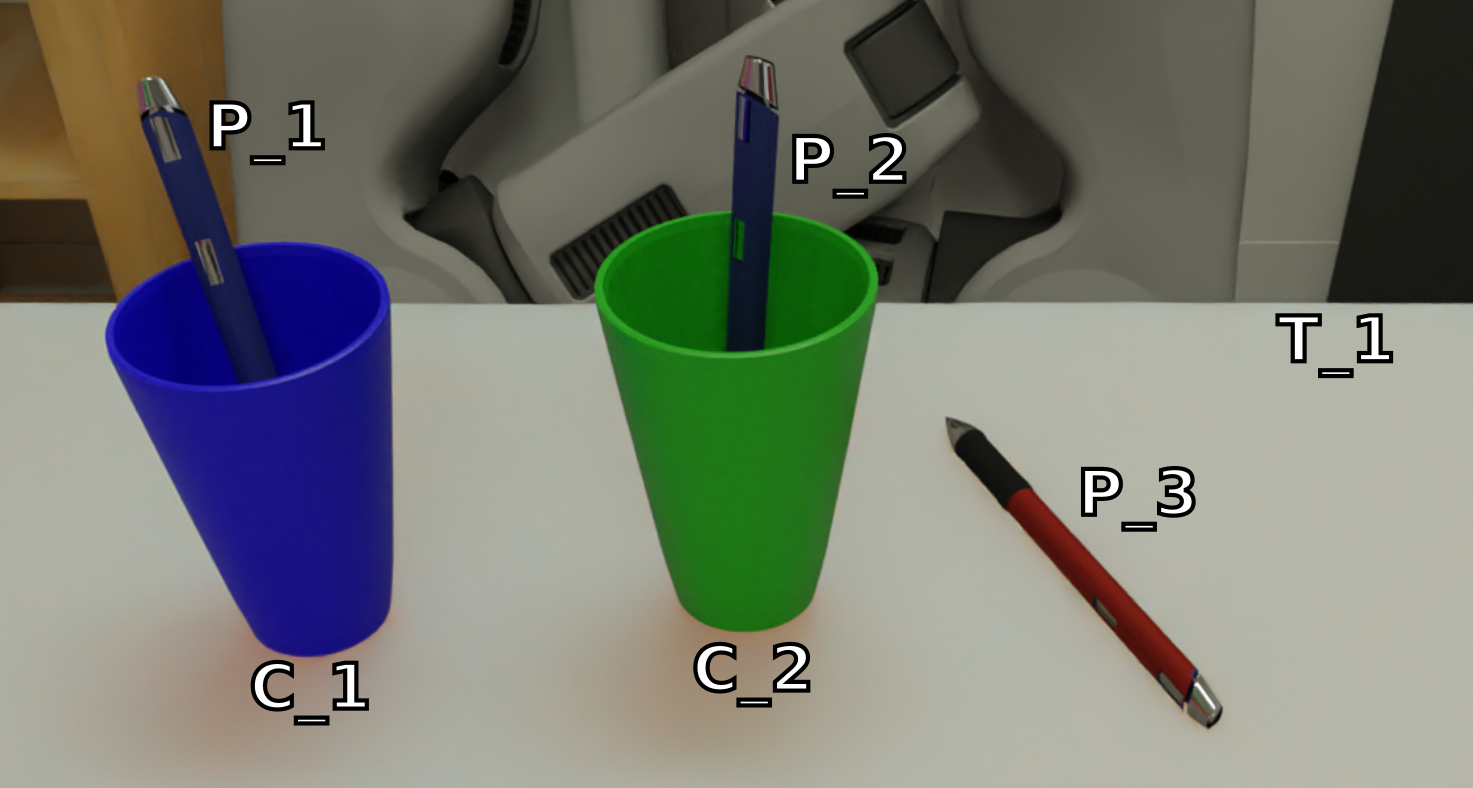
\includegraphics[scale=0.2]{figures/chapter4/pens.png}
\caption{\label{fig:chap4_kb} A situation view from the hearer perspective, with the robot placed on the other side of the table. Three pens and two cups are on a table. The two blue pens are each in one cup. }
\end{figure}

In this chapter, we take as an example the situation represented in Figure~\ref{fig:chap4_kb}. The situation is assumed to be perceived by the robot and represented in its semantic knowledge base. This knowledge base as an ontology is of the form $\kbs^R = \langle \Abox^R, \Tbox^R, \Rbox^R \rangle$. $\Abox$, $\Tbox$ like presented in Section~\ref{sec:kb_formalism}. The estimated knowledge base of the human partner $\kbs^H$ is here assumed to be the same as that of the robot in the way that $\kbs^R \equiv \kbs^H \equiv \kbs$.

The TBox used to describe the situation of this example is represented in figure~\ref{fig:chap4_kb_Tbox}. The class IkeaLisabo represents a precise model of tables and does not have any label. The class Pen is specified through two classes the ClickingPen and the TurningPen. These two classes aim at representing the pens you need to click on top to get the tip of the pen out and the pens you need to turn to get the tip of the pen out. These classes do not have any label to directly speak about them. They are only used by the robot to know how to use them. For sure a more precise ontology could be drawn but we try to keep it simple for the purpose of this chapter.

\begin{figure}[h!]
\centering
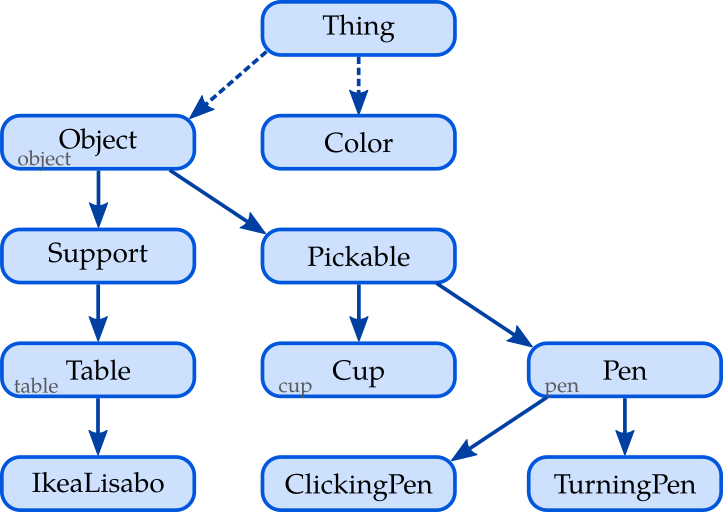
\includegraphics[scale=0.4]{figures/chapter4/pens_Tbox.png}
\caption{\label{fig:chap4_kb_Tbox} Representation of the TBox (classes hierarchy) used to describe the situation of the Figure~\ref{fig:chap4_kb}. }
\end{figure}

The ABox used to describe the situation is represented in Figure~\ref{fig:chap4_kb_Abox}. The two cups C\_1 and C\_2 are on the table T\_1. The two pens P\_1 and P\_2 are respectivly in the cups C\_1 and C\_2 while P\_3 is directly on the table. The pen P\_4 is another pen, not on the table. Other objects could be represented as the robot and the human could know other object being in the room. The pen P\_1 is the only pen for which the agent has to click to get the tip of the pen out.

\begin{figure}[h!]
\centering
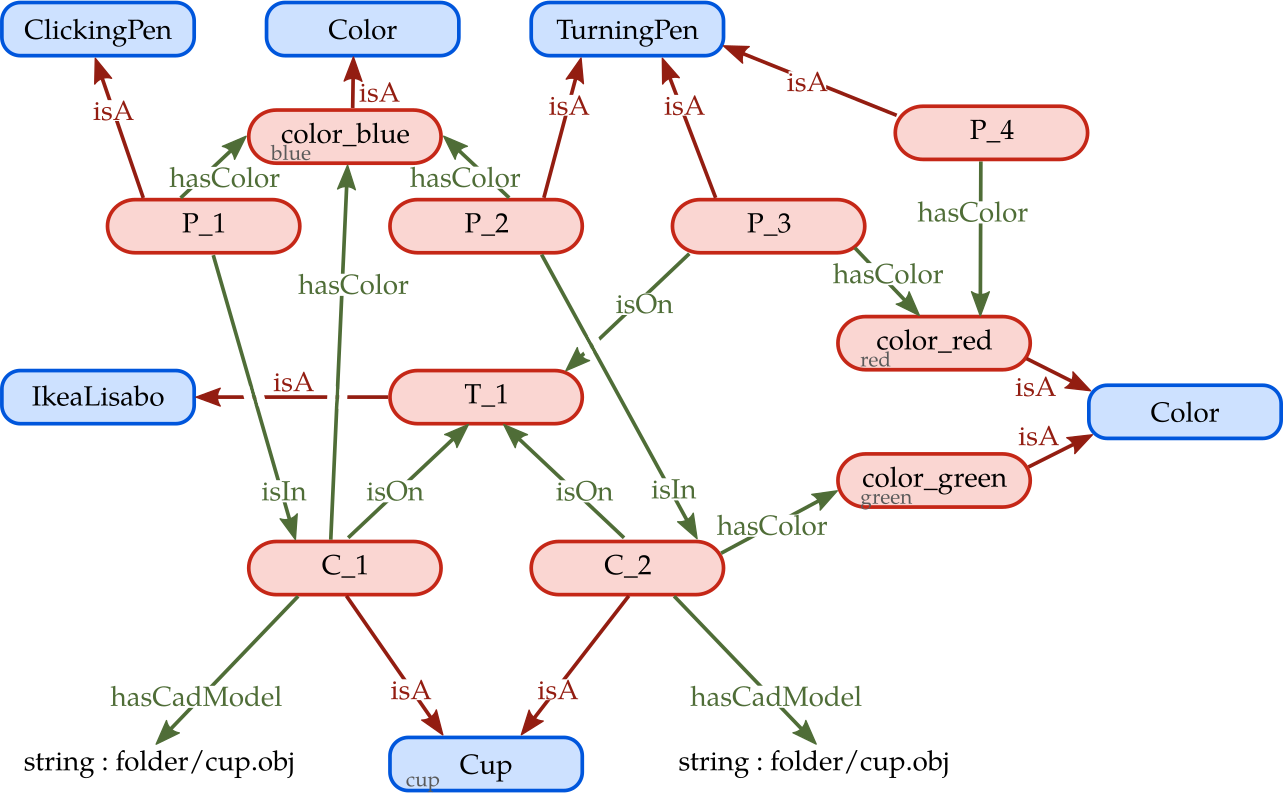
\includegraphics[scale=0.38]{figures/chapter4/pens_Abox.png}
\caption{\label{fig:chap4_kb_Abox} Representation of the ABox (relation graph) used to describe the situation of the Figure~\ref{fig:chap4_kb}. }
\end{figure}

The RBox is not represented but the properties composing it are the ones used in the ABox. In addition we define the properties \textit{hasIn} being the inverse of \textit{isIn} and \textit{isUnder} being the inverse of \textit{isOn} ($\{(isIn,\ hasIn), (isOn,\ isUnder)\} \subset \invset$). Moreover, the property \textit{isOn} inherits of the upper property \textit{isAbove} ($\{(isOn,\ isABove), (isUnder,\ isBelow)\} \subset \inclset$). While the first defines a direct contact between two entities, the other does not. Finally, we declare the chain axiom: $isIn \bullet isOn \Rightarrow isABove$. This axiom allows to reason on the ontology and declare that if a first entity is in a second one and that this second is on a third one, the first entity is above the third. Taking our example, because P\_1 is in C\_1 that is on T\_1, the pen P\_1 is above the table T\_1.

\subsection{Contextualization and restriction for situated REG}

The human (named Tony) and the robot are involved in a shared task around a table. During the task, the robot needs a blue pen to write. However, it can not take one by itself as the blue pens are in cups. Moreover, with its huge gripper, it can not use the kind of pens where you have to click. Our robot thus precisely need the pen P\_2 of our example and has to ask it to its human partner\footnote{Some could tell that if it is not the first time that our robot and this human collaborate, the human could be aware of the robot capabilities. In this case, the robot would just have to ask for a blue pen and the task would be over. We thus consider that our robot never had interacted with this particular human. For sure it could explain its capabilities but the purpose is not there.}.

The robot is thus aiming to unambiguously designate a specific entity $\goalindiv \in \indivset$, called the \textbf{target entity}, through its attributes and relations to other entities. However, as explained, the \acrshort{reg} is meant to be used in the context of an upper task that has to be taken into account. In our example, the collaborative task concerns objects on the table so that the other entities in the room are clearly out of context. Asking for a pen, P\_4 will not lead to an ambiguous situation as it is not on the table around which the interaction is performed. To represent this restriction, we provide the problem a \textbf{context} $Ctx = (\relationset_{ctx}, \inheritset_{ctx})$. It is a set of relations and direct types that are implicit in the current communication with regard to the task. This context is used to find a reference to $\goalindiv$, but has not to be included in the generated \acrshort{re}. For our example the context could be $Ctx = (\{ (\goalindiv,\ isAbove,\ T\_1), (\goalindiv,\ isVisibleBy,\ Tony) \},\ \emptyset)$. With this context, we state that the entity to refer to (i.e. $\goalindiv$) is known to be above the table T\_1 and visible by the human partner, Tony. Because $isAbove$ is an upper property of $isOn$, all entities on the table are concerned. Moreover, thanks to the chain axiom, any entity being in an entity on the table are also concerned. The direct types in the context could be used in a more complex communication in which we already know that we are speaking about a pen.

In addition to the entities being out of the context and thus not taken into account, some relations might be present in the knowledge base, but cannot be used in a communication process. In our example, the relations using the \textit{hasCadModel} property should not be used as the robot cannot communicate them verbally. To represent this restriction, we provide the problem a set of so-called \mbox{\textbf{usable properties}} $\usablepropset \subseteq \propset$. Any relation involving as predicate a property that is not part of the usable properties set can, therefore, not be used in the solution. Because of properties inheritance, $Incl$ all the properties inheriting from the ones in $\usablepropset$ are consequently usable to solve the problem. 


With regard to the presented restrictions, the \acrshort{reg} problem is define as follow:

\begin{definition}[Referring Expression Generation problem]
The \acrshort{reg} problem is a tuple $\problem = \langle \goalindiv, \kb, Ctx, \usablepropset \rangle$ with $\goalindiv \in \indivset$ the target entity, $\kbs$ the hearer semantic knowledge base, $Ctx$ the \acrshort{re} context, and $\usablepropset \in \propset$ the usable properties.
\end{definition}

A representation of the ABox on which the restrictions have been applied\footnote{We do not create a second ABox with the only elements that can be used. The \acrshort{reg} algorithm will have to manage the restrictions during the search process. Otherwise, we lost the interest to run on a knowledge base common to the entire robotic architecture.} is represented in Figure~\ref{fig:chap4_kb_ctx}.

\begin{figure}[h!]
\centering
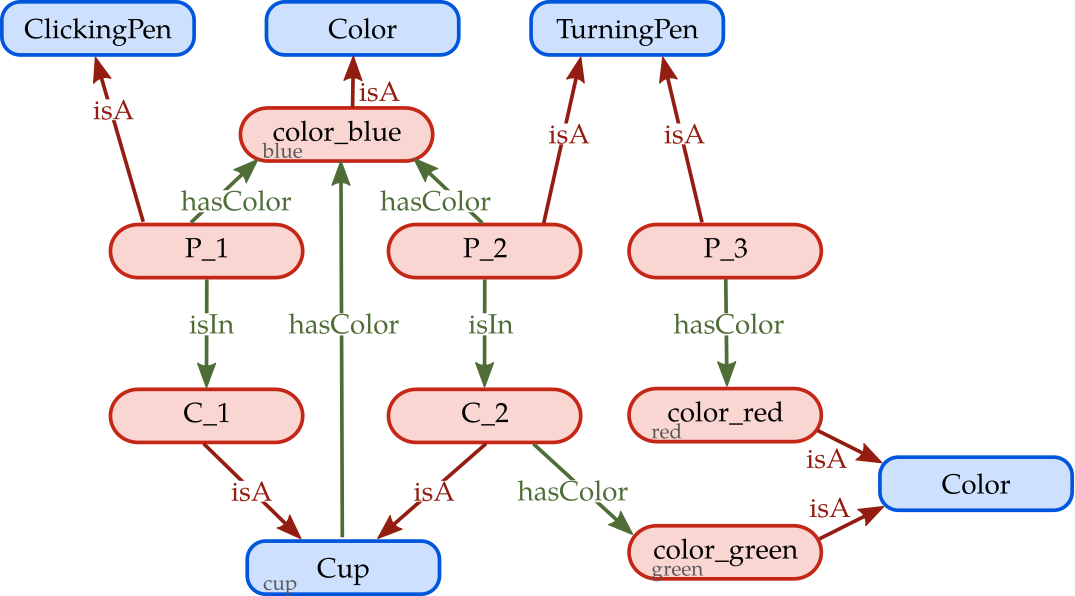
\includegraphics[scale=0.38]{figures/chapter4/pens_ctx.png}
\caption{\label{fig:chap4_kb_ctx} Representation of the ABox (relation graph) on which the context of the problem and the usable properties have been applied. }
\end{figure}

\subsection{Expected solution: structure and validity criteria}

What we might expect from a \acrshort{reg} solver would be to generate a natural language sentence. However, as explained earlier, we focus here on the sub-task that is the content generation rather than the linguistic realization. For the content generation, the attempted solution is often a set of relations like $\{ (\goalindiv,\ hasColor,\ red)\}$. The issue of such a set is that it can not be verbalized afterwards. Indeed, some entities are not labelled and thus can not be used directly in the solution. In our example, it the case for the three pens $P\_1$, $P\_2$, and $P\_3$. They are what we called \textbf{anonymous entities}. To refer to an anonymous entity and be able to speak about it we must pass at least by its type. This is what we naturally do when we say \textit{``the red pen''} where the concept \textit{``pen''} does not directly refer to the entity but rather to its type. Before going ahead in the definition of the form of the solution, we can already set a constraint on its content through \textbf{the parlance need}.

\begin{theorem} [The parlance need]
\label{the:parlance_need}
For any entity appearing in a \acrshort{re}, exactly one naming relation must be added.
\end{theorem}

What we call a naming relation is in its simplest form the presence of a label. The relation to add is thus of the form: $(\indiv_t,\ hasLabel,\ ``tony'')$. In the case an entity does not have any label, we pass by one of its type which has a label: $\{(\indiv_t,\ isA,\ Pen), (Pen,\ hasLabel,\ ``pen'')\}$. This type is not necessarily the direct type of an entity. It could be an inherited one if needed.

Let us now introduce $\varset$, a set of variables. Because anonymous entities are not directly present in the \acrshort{re} sentence (hence the presence of ambiguities), we will replace all of them with variables. They are prefixed with a question mark. The set $\varset$ thus keep a track of these variables. Taking the example of the red pen and replacing the anonymous entities by their corresponding variable, the set of relation become: \textit{\{(?0, isA, Pen), (Pen, hasLabel, ``pen''), (?0, hasColor, red), (red,  hasLabel, ``red'')\}}. Because anonymous entities are now represented by variables, the relations representing the labels can be removed as it is implicit that the others have one. The reference is thus \textit{\{(?0, isA, Pen), (?0, hasColor, red)\}} that is exactly of the form of a \sparql{} query.

\begin{definition}[Referring expression]
A referring expression is a set of underspecified relations of the form of $(s, p, o) \in (\varset \cup \indivset) \times \propset \times (\varset \cup \indivset)$ or $(s, isA, o) \in \varset \times ``isA'' \times \classset$ for type ascription.
\end{definition}

The form of the wanted solution would thus be as a \sparql{} query. It can easily be built from a set of relations. All the content information are present in it, in addition to the representation that some entities can not be verbalized directly. The way to resolve a \sparql{} query can be compared to the process we perform as human to understand a \acrshort{re}. We search all the combination of entities matching the \acrshort{re}. We can thus define the \textbf{correct instantiation} constraint.

\begin{theorem} [The correct instantiation]
\label{the:correct_intance}
For any variable appearing in a \acrshort{re}, a least one substitution function $f: \varset \rightarrow \indivset$ must exist.
\end{theorem}


\begin{table}[htb!]
\resizebox{\textwidth}{!}{%
\begin{tabular}{|l|l|l|l|l|l|}
\hline
 &
  \textbf{Target} &
  \textbf{Relations set} &
  \textbf{sparql query} &
  \textbf{Sentence} &
  \textbf{Instantiations} \\ \hline
a) &
  P\_3 &
  \begin{tabular}[c]{@{}l@{}}\{(P\_3, isA, Pen),\\ (P\_3, hasColor, red)\}\end{tabular} &
  \begin{tabular}[c]{@{}l@{}}\{(?0, isA, Pen),\\ (?0, hasColor, red)\}\end{tabular} &
  The red pen &
  {[}?0 =\textgreater P\_3{]} \\ \hline
b) &
  P\_2 &
  \begin{tabular}[c]{@{}l@{}}\{(P\_2, isA, Pen),\\ (P\_2, isIn, C\_2)\\ (C\_2, isA, Cup)\}\end{tabular} &
  \begin{tabular}[c]{@{}l@{}}\{(?0, isA, Pen),\\ (?0, isIn, ?1)\\ (?1, isA, Cup)\}\end{tabular} &
  \begin{tabular}[c]{@{}l@{}}The pen in\\ the cup\end{tabular} &
  \begin{tabular}[c]{@{}l@{}}{[}?0 =\textgreater P\_2,\\ ?1 =\textgreater C\_2{]},\\ {[}?0 =\textgreater P\_1,\\ ?1 =\textgreater C\_1{]}\end{tabular} \\ \hline
c) &
  P\_2 &
  \begin{tabular}[c]{@{}l@{}}\{(P\_2, isA, Pen),\\ (P\_2, isIn, C\_2),\\ (C\_2, isA, Cup),\\ (C\_2, hasColor, green)\}\end{tabular} &
  \begin{tabular}[c]{@{}l@{}}\{(?0, isA, Pen),\\ (?0, isIn, ?1),\\ (?1, isA, Cup),\\ (?1, hasColor, green)\}\end{tabular} &
  \begin{tabular}[c]{@{}l@{}}The pen in\\ the green cup\end{tabular} &
  \begin{tabular}[c]{@{}l@{}}{[}?0 =\textgreater P\_2,\\ ?1 =\textgreater C\_2{]}\end{tabular} \\ \hline
\end{tabular}%
}
\caption{Three referring expressions extracted from the example of Fig.~\ref{fig:chap4_intro}. For each target, is represented the relations set, the equivalent \sparql{} query, the corresponding sentence in natural language, and the possible instantiations.}
\label{tab:REs}
\end{table}

Examples of REs base on the Figure~\ref{fig:chap4_intro} are presented in Tab.~\ref{tab:REs}. All three respect the constraints of theorems~\ref{the:parlance_need} and \ref{the:correct_intance}. However, the example b) does not refer in an unambiguous way the entity P\_2. We thus define the two \acrshort{re} validity constraints.

\begin{theorem} [The RE minimal validity]
\label{the:re_mini_validity}
A \acrshort{re} is said to be minimally valid iif the variable $\var_t \in \varset$ representing the target entity $\goalindiv$ has only one possible instantiation being $\indiv_t$ itself.
\end{theorem}

\begin{theorem} [The RE complet validity]
\label{the:re_compl_validity}
A \acrshort{re} is said to be completely valid iif it is minimally valid and if for all the variables $\var \in \varset$ involve in the \acrshort{re}, each has only one possible instantiation.
\end{theorem}

Taking the example of the Figure~\ref{fig:chap4_complet} where the goal of the situation is to refer to cup B, it can be achieved in two manners. Asking for the cup with a pen inside is a referring expression said to be minimally valid as the referred pen is ambiguous. However, not solving this ambiguity between the two pens in the cup still allow identifying the referred cup. To make the solution to be completely valid, we should ask for the cup with the red pen inside or the cup with the blue pen inside\footnote{A minimally valid reference can thus use references to set of entities. This is not an issue but the linguistic realisation should take it into account using ``a'' rather than ``the'' (e.g. ``with a pen inside'' rather than ``with the pen inside'').}.

\begin{figure}[h!]
\centering
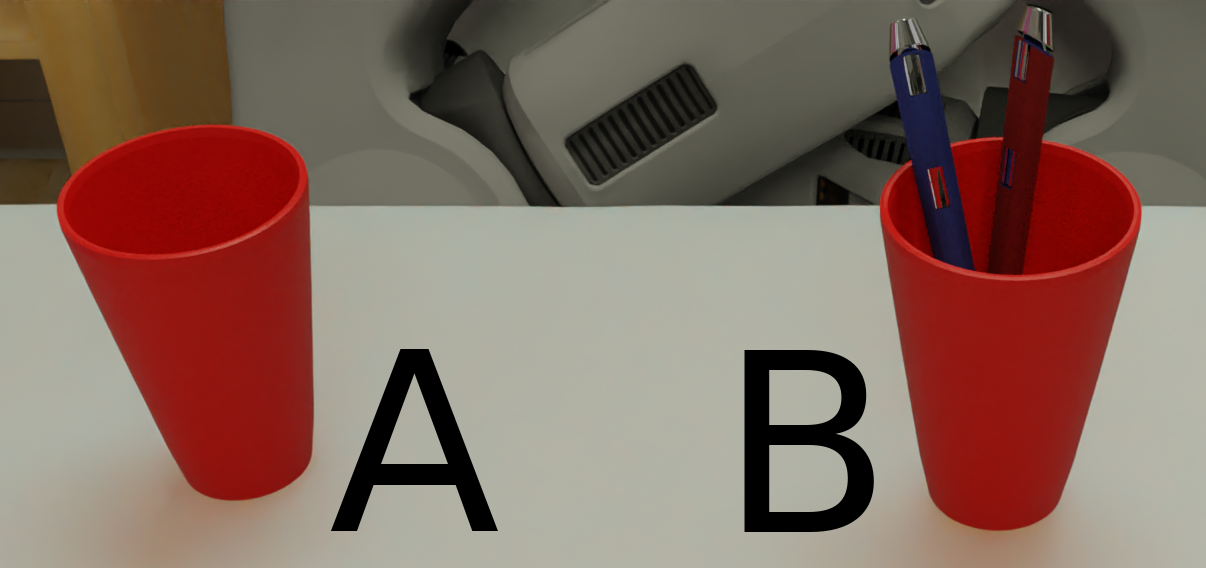
\includegraphics[scale=0.15]{figures/chapter4/complet_validity.png}
\caption{\label{fig:chap4_complet} A situation where referring to the cup B through realtions to the pens can be done either by leaving the ambiguity on the pen (minimally valid \acrshort{re}) or also disambiguating the color of the pen (completely valid \acrshort{re}). }
\end{figure}

With regard to the presentend constraints, a solution to a \acrshort{reg} problem is define as follow:

\begin{definition}[Referring Expression Generation solution]
A solution to the \acrshort{reg} problem is thus $\solution = \langle E, \var_t \rangle$, with $E$ a valid referring expression in the form of a set of under-specified relations representing the \sparql{} query and $\var_t$ the variable designating the target entity $\goalindiv$.
\end{definition}


Finally, considering the fact that some relations are easier to understand than others, we can define the relations cost function\footnote{The cost function is here seen as a black-box which can be a static map, the result of a learning process or other.} $\costfunc : \relationset \rightarrow \mathbb{R}^+$. Thanks to it, we can define an optimal solution to a \acrshort{reg} problem.

\begin{definition}[Optimal Referring Expression Generation solution]
The optimal solution $\solution^* = \langle E^*, \var_t \rangle$ is thus the solution minimizing $\sum_{\relation \in E^*} \costfunc(\relation)$ over the set of all the possible solutions for a \acrshort{reg} problem.
\end{definition}


\section{Uniform Cost Search REG}

In the previous section, we have defined a Referring Expression Generation problem as well as its solution. In this section, we first formalise this problem as a search problem and we then present an algorithm abe to solve it in a smart way.

\subsection{Formalisation as a search problem}

In the \acrshort{reg} problem, we can consider a \textbf{candidate Referring Expression} as a \textbf{state} $\state$ of a search algorithm. A candidate \acrshort{re} is a \acrshort{re} under construction that does not respect all the constraints to make a valid \acrshort{re}. It is a set $\mathcal{T} \subseteq \relationset \cup C$ of relation $\relation$ representing relations present in the referenced knowledge base $\kbs$. The \textbf{initial state} is specified by the context of the problem that is a set of relations that we assume to be already known by the hearer.
%\footnote{If you do not understand why we use a set of relations while we said that a \acrshort{re} in a set of under-specified relations in the form of a $\sparql{}$ query, just remember that we can easily go from one to the other.}

To find all the entities referred by a candidate \acrshort{re}, we transform it into a \sparql{} query by replacing the anonymous entities with variables. We then submit it to the ontology to know which entities can be bound to each variable of the query. Depending on whether the result of the query gives the correct matches between variables and entities or not, we can know if a state is a \textbf{target state} or not. A state is a target state if the matching between the variables and the entities make the \acrshort{re} valid (minimally or completely regarding our needs).

An \textbf{action} $\action$ in the \acrshort{reg} problem consists in the insertion of a new triplet $(\subject, \property, \object)$ to the set $\mathcal{T}$ of a state $\state$. Performing an action on state results in the creation of a new state $\state'$. The inserted triplet can represent an entity type (coming from $\inheritset$) or a relation between entities (coming from $\relationset$). When it represents an entity type, we call the action a \textbf{typing action} with $\property \equiv isA$. When it is a relation coming from the relation set $\relationset$, we want it to reduce the existing ambiguity in a given state. We thus expect the relation to differ between ambiguous entities in $\state$. In this case, we call the action a \textbf{difference action}. To consider the open-world assumption, we can refine this difference in two categories:

\begin{definition}[Hard difference]
A hard difference exists when two ambiguous entities own the same property towards a different entity: $(\indiv_i, \property, \object_i) \in \relationset \land (\indiv_j, \property, \object_j) \in \relationset | \object_i \neq \object_j$. We note this difference between two entities ($\indiv_i, \harddiff, \indiv_j$).
\end{definition}

\begin{definition}[Soft difference]
A soft difference exists when an entity owns a property that is not owned by another ambiguous entity: $(\indiv_1, \property, \object_i) \in \relationset \land (\indiv_j, \property, \cdot) \notin \relationset$. We note this difference between two entities ($\indiv_i, \softdiff, \indiv_j$).
\end{definition}

Considering the Figure.\ref{fig:chap4_complet} with the two pens, it exists a hard difference between the two pens regarding their color as one is blue and the other is red. The two pens own a relation with the same property \textit{hasColor} but on different entities, red and blue. A soft difference exists between the two cups as cup B has something inside and not cup A.

To represent the fact that some referring expressions are easier to understand than others depending on the property they use, we define a \textbf{cost} for each state. It is the sum of the cost of the properties used in the relations composing the candidate \acrshort{re}. The cost can thus be regardless assigned to the property of the relation or the relation itself and the cost of an action is the cost of the relation it inserts. If we assume a state $\state$ with a cost $\cost$, performing an action $\action_j$ corresponds to the fact of adding a relation $\relation_j$ and create a new state $\state'$. The cost of this new state can be calculated either from the cost of the previous state $\cost' = \cost + \costfunc(\relation_j)$ or independently $\cost' = \sum_{\relation \in \mathcal{T}} \costfunc(\relation)$. In addition, as the hard differences respect the open-world assumption while the soft differences do not, we propose to encourage the use of hard difference when possible by adding an extra cost to relations coming from soft differences.

To manage the \acrshort{reg} problem as a search problem, we finally define a search \textbf{node} $\node$ that is, at least, composed of a candidate \acrshort{re} (thus a state) $\state$ and a cost $\cost$.

\subsection{Algorithm choice}

We consider the \acrshort{reg} problem to be a graph search problem when we perform it on an ontology. If we had considered a state $\state'$ as being composed only of the relation provided by the action $\action$ from state $\state$, a tree search should have been used because state $\state'$ would depend on state $\state$. Considering a state as being a set $\mathcal{T}$ of relations $\relation$, the states become independent of each other and can be compared as $\mathcal{T}_x = \mathcal{T}_y$ iff $\forall{z},(z\in \mathcal{T}_x \Leftrightarrow z\in \mathcal{T}_y)$.

From any state, we can compute the number of pending ambiguous entities. We could think that this knowledge beyond the problem definition could be used to drive the search. However, when we say that it still has X ambiguous individuals this means that the algorithm will have to perform at most X actions to reach a target state. This means that the heuristic function would overestimate the cost to reach the goal. In this sense, such a heuristic is not admissible and informed search is not applicable.

Although we could define the reverse actions that is to remove relations from a state, we do not know any solution of the problem and therefore we cannot do a backward search from it.

Taking a look to breath-first search, it is optimal when all steps costs are equal because it always expands the shallowest unexpanded node. However, in the \acrshort{reg} problem, actions do not have the same cost as explained previously to represent the preference over features. In this case, the breadth-first search is not optimal and is therefore not suited to our problem.

At the difference of the breadth-first search, the \textbf{\acrfull{ucs}} expands the node with the lowest cost. That allows us to take advantage of the preference over features to find efficiently the optimal solution. Indeed, it is \textbf{optimal} and \textbf{complete} with positive action costs and a finite number of entities and properties in $\kb$.

\subsection{Algorithm presentation}

\begin{algorithm}[ht!]
\caption{Uniform-Cost Search algorithm for Referring Expression Generation}
\label{alg:chap4_ucs}
\begin{algorithmic}
\Function{UCS\_REG}{$problem$} 
    \State $node\leftarrow$ a node with RE = \textsc{create-initial-re}(\textit{problem}.context), \textit{cost} = 0
    \State $frontier\leftarrow$ a priority queue of nodes ordered by their \textit{cost}
    \State $frontier\leftarrow$ \textsc{INSERT}($node$, $frontier$)
    \State $explored\leftarrow$ an empty set
    \\
    \Loop
        \If{\textsc{empty}($frontier$)} 
        	\State \Return failure
        \EndIf
        \\
        \State $node\leftarrow$ \textsc{pop}($frontier$)
        \If{\goaltest($problem$, \toquery($node$))} 
        	\State \Return \textsc{SOLUTION}($node$)
        \EndIf
        \\
        \State add $node.RE$ to $explored$
        \ForAll{$action$ in \actions($node$)}
            \State $child \leftarrow \createchild(node, action)$
            \If{$child.RE$ is not in $explored$ or $frontier$}
            	\State $frontier\leftarrow$ \textsc{INSERT}($child$, $frontier$)
            \EndIf
        \EndFor
    \EndLoop
\EndFunction
\end{algorithmic}
\end{algorithm}

Our \acrshort{reg} algorithm performs a graph search in the space of states, using the \acrlong{ucs} algorithm presented in Algorithm~\ref{alg:chap4_ucs}.
From an initial state, built from the context of the query, the algorithm generates a set of actions that add relations to the current state and create new states to explore. Just like Dijkstra's algorithm, it expands the states in increasing cost order until a solution is discovered or the search space is exhausted. We can however note a slight difference with the original algorithm. In our case, we know that two candidates \acrshort{re} said to be equivalent (i.e. owning the same relations regardless of their order) always have the same cost. Consequently, we do not need to replace in the frontier a node with an equivalent state but having a higher cost than the newly created child node.

We will now detail the functions specific to the \acrshort{ucs} applied to the \acrshort{reg} problem.

\textbf{\tovariable: }
We globally define a symbol table $\symboltable$ to keep track of the variables assigned to the anonymous entities. When a new anonymous entity is found, it is inserted in this symbol table with a unique variable identifier. We note $\symboltable^{-1}$ the inverse table, allowing us to retrieve the entity represented by an existing variable.

\textbf{\toquery: }
It performs the translation of a set of triplets into a \sparql{} query. To do so, each anonymous entity has to be replaced by its corresponding variable. For each entity involved in the set of triplet to convert, they are given aN UTF8 string representation with the function $v(\indiv): \indivset \mapsto str$: 
\[ 
    v(\indiv) = 
    \begin{cases}
        str(\indiv),& \text{if } \alabel(\indiv) \neq \emptyset\\
        \symboltable(\indiv),& \text{otherwise}
    \end{cases} 
\]

\textbf{\sparqlresult: }
It takes a \sparql{} query as input and returns a match table $\matchtable$ in the way that $\matchtable(\var)$ is the set of entities matching the variable $\var$ in the given query. While usually the matching entities of a given variable depend on the matching entities of another one\footnote{See the example b of table~\ref{tab:REs} for an illustration of this link.}, we do not need to keep this link in our application.

\textbf{\goaltest: }
The test first fails if not all the anonymous entities involved in the tested candidate \acrshort{re} are typed. If this first test succeeds, the function succeeds, for a minimally valid solution, if the target entity $\goalindiv$ is the only solution to the variable $v(\goalindiv)$ in $\matchtable$. For a completely valid solution, the test succeeds if the previous test succeeds and if all the others variables of $\matchtable$ have exactly one solution.

\textbf{\createchild: } 
Creating a child node from a parent node and an action is easy to see. The \createchild function is specified in the pseudo-code of Algorithm \ref{alg:child}. 

\begin{algorithm}[H]
\caption{\label{alg:child} Child node function pseudocode}
\begin{algorithmic}
\Function{\createchild}{$action$, $parent$} 
    \State \Return a node with
    \State RE = $parent$.RE $\cup$ $action$
    \State cost = $parent$.cost + $\costfunc(action)$
\EndFunction
\end{algorithmic}
\end{algorithm}

\textbf{\actions: }
For each explored state, we consider two kinds of possible actions that we can perform on it. First, the \typingactions{} aims at proposing the addition of inheritance relations for all the anonymous entities for which no inheritance relation exists in $\mathcal{T}$. Second, the \differenceactions{}, divided into \textbf{hard difference actions} and \textbf{soft differences actions}, consists in the addition of relations that differ between the ambiguous entity for each variable in $\matchtable$.

In the \typingactions{} function (Alg.~\ref{alg:typing_action}), the function \textsc{UsableClasses} returns the most specific \textit{labeled} classes of an entity $\indiv$. In other words, it returns the set of classes $\class \in \classset$ such that $(\indiv,\class) \in C$, $\tlabel(\class) \neq \emptyset$, and
$\not\exists \class'\ s.t.\ (\class', \class) \in H \wedge \tlabel(\class') \neq \emptyset$.

\begin{algorithm}[htb!]
\caption{\label{alg:typing_action} Typing actions pseudocode}
\begin{algorithmic}

    \Function{\typingactions}{$state$} 
        
        \ForAll{$(\subject, \property, \object)$ \textbf{in} $state$}
            \If {$\alabel(\subject) = \emptyset\ \wedge \not\exists \class \text{~s.t.~} (\subject, $``isA''$,\class) \in \textit{state}$}
                \State \Return $\{\ (\subject,\text{``isA''},t)\ |\ t \in \textsc{UsableClasses}(\subject)\  \}$
            \ElsIf {$\alabel(\object) = \emptyset\ \wedge \not\exists \class \text{~s.t.~} (\object, $``isA''$,\class) \in \textit{state}$}
                \State \Return $\{\ (\object,\text{``isA''},t)\ |\ t \in \textsc{UsableClasses}(\object)\  \}$
            \EndIf
        \EndFor
        \Return OK \Comment{every anonymous entity is typed}
    \EndFunction
\end{algorithmic}
\end{algorithm}

The choice to select the most specific class differs from the one of \cite{dale_1995_computational} that prefers the least specific types also called the basic-level classes. However, using a knowledge base not specific to the \acrshort{reg} task, it would always return the classes \textit{Object} or \textit{Thing}. This could lead to confusion for the hearer and would not help to reduce the ambiguity with other entities. Selecting the most specific thus reduces the branching factor of the algorithm as soon as possible and does not impacts the completeness. Moreover, working on the estimated knowledge base of the \acrshort{re} hearer, we can assume that the used labels and thus concepts are known to the hearer.

The \typingactions{} is always performed before the \differenceactions{} and this second is even not called if the first has found possible actions. We thus ensure that we do not have more than one untyped anonymous entity at the time. This particularity explains why the \typingactions{} stops at the first untyped anonymous entity. Besides, it reduces once again the branching factor. Because of the parlance need constraint, we knew that any untyped anonymous entity has to be typed to find a valid solution. It is thus useless to try to add other relations while such an entity still exists in a candidate \acrshort{re}. Even if, for any reason, we found ourselves in a case with multiple untyped anonymous entities at the time, each of them will be typed after the other\footnote{Typing them at once would reduce the execution time but would necessitate actions to be the insertion of a set of relations which add complexity to the algorithm for cases that should not append.}.

\begin{algorithm}[htb!]
\caption{\label{alg:diffeaction} Hard difference actions pseudocode}
\begin{algorithmic}[1]
\Function{\textsc{HardDifferenceActions}}{$state$} 
    \State $actions\leftarrow$ an empty set of actions
    \State $matches\leftarrow$ \sparqlresult(\toquery($state$))

    \ForAll{$(\var, \indiv)$ \textbf{in} matches}
        \If{$\indiv \neq \symboltable^{-1}(\var)$}
            \ForAll{$r = (\symboltable^{-1}(\var), p, o)$ \textbf{in} $\symboltable^{-1}(\var) \harddiff \indiv$} 
                \State $r_{inv}$ = $(o, Inv(p), \symboltable^{-1}(\var))$
                \If{$r \not\in state \wedge r_{inv} \not\in  state \wedge p\in U$}
                    \State $\textit{actions} \gets \textit{actions} \cup \{r\}$
                \EndIf
            \EndFor
        \EndIf
    \EndFor
    \Return $actions$
\EndFunction
\end{algorithmic}
\end{algorithm}

The \differenceactions{} function call consecutively the hard then soft differences actions functions and merge their results. The pseudo-code of the hard difference actions function is provided in Algorithm~\ref{alg:diffeaction}. The $\harddiff$ at line 6 (resp. $\softdiff$) operator returns all the relations that are hard differences (resp. soft) between two entities. In both cases, an action can be added only once and must not be present in the current state to avoid redundancy. Moreover, an action can not be added if the inverse relation to the one added is already present in the current state or proposed actions. We use the $\invset$ set defined in the knowledge base to check it. It once again avoids any redundancy. Taking the example of Figure~\ref{fig:chap4_kb}, the relation $(C\_1, isOn, T\_1)$ would be redundant if the relation $(T\_1, isUnder, C\_1)$ has been already used in the current candidate \acrshort{re}.

\subsection{Replanning and explaining failures}

When the hearer does not understand the referring expression, we could either repeat exactly the same sentence or be smarter and add more information than needed to help him. To do so, slight modifications have to be made to the current algorithm. In the case of replanning, the frontier and the explored set do not have to be re-initialized and in case of success, the current node has to be inserted in the explored set and the next possible actions to be found before exiting. These simple modifications are sufficient to refine a not understood \acrshort{re}.

When no referring expression can be found, it could be interesting to give more information about the failure to the upper process. In the case of the \acrshort{reg} problem, it could be to give the entities still in ambiguity. With such information, an upper deliberative process could in this way act on these entities to remove the ambiguity. To do so, we just have at each step of the algorithm, to keep a track of the node having the minimum of ambiguous entities. This information is present in the matching table $\matchtable$ for each node.

\section{Results}

In this section, we present the solution found by our algorithm on the example presented in section~\ref{sec:chap4_kb}. We then challenge our algorithm on a large scale ontology representing a three-room apartment to analyse it in terms of time execution, solution length and composition. Finally, we provide comparisons with two state-of-the-art methods on their own domains.

\subsection{Solution analysis: The pen in the cup}

To familiarize with the form of the solutions and better understand how the algorithm constructs them, we first solve the example of Figure~\ref{fig:chap4_kb}. The target entity $\goalindiv$ is P\_2. The corresponding variable $\var_t$ in the \sparql{} query is denoted $?0$. We assume the general knowledge to be the Tbox of Figure~\ref{fig:chap4_kb_Tbox} and the perceived relations to be the ABox of Figure~\ref{fig:chap4_kb_Abox}.

The context of the problem is that we are speaking about objects being above the table T\_1: $Ctx = (\{(?0,\ isAbove,\ T\_1)\}, \emptyset)$. The usable properties are $\usablepropset = \{visualProp,\ geometricProp\}$. Because of the properties inclusions, the properties \textit{isIn}, \textit{hasIn}, or \textit{hasColor} are usable. The problem is thus define by $\problem = \langle P\_2, \kbs, Ctx, \usablepropset \rangle$.

Since the classes \textit{ClinkingPen} and \textit{TurningPen} do not have labels, the lowest labelled class of P\_1, P\_2, and P\_3 is \textit{Pen}. A recall of the situation and the available knowledge base on which the context and the usable properties have been applied is represented on the top of Figure~\ref{fig:chap4_search}.

\begin{figure}[h!]
\centering
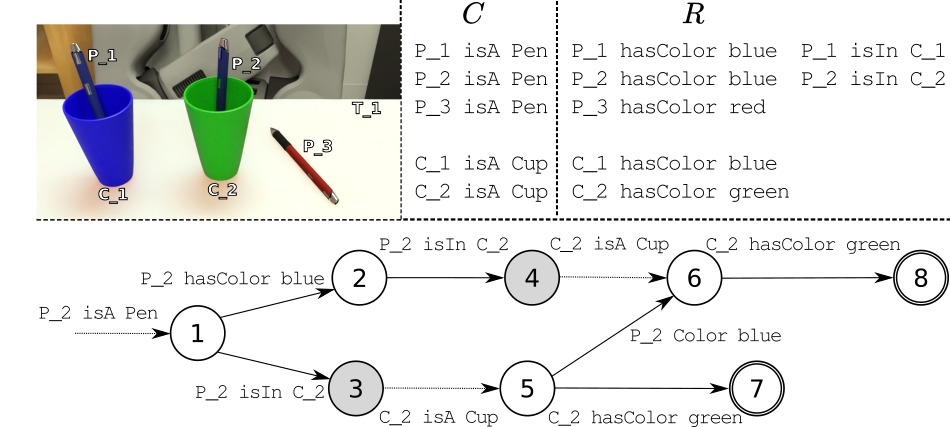
\includegraphics[scale=0.45]{figures/chapter4/search.png}
\caption{\label{fig:chap4_search} On top, a recall of the situation of Figure~\ref{fig:chap4_kb} and the entities types and relations.
At the bottom, a graphical representation of the search progress to generate a referring expression to the entity P\_2. Numbers represent the order in which the nodes are explored. Arrows are the actions performed on the nodes. Hashed arrows correspond to typing actions and greyed nodes do not respect the parlance need constraint. Double circled nodes are valid nodes. }
\end{figure}

The search process is represented at the bottom of Figure~\ref{fig:chap4_search}. It starts with node 0 in which we know that P\_2 is above the table. In this node, P\_2 is an anonymous entity and is not typed. The only possible action is thus to type it, creating node 1 with the candidate \acrshort{re} $\{(?0,\ isA,\ Pen)\}$. From this node, two difference actions are created and two new nodes are generated. Because the action leading to node 3 introduces a new anonymous entity, it also introduces a new variable to represent it. The candidate \acrshort{re} related to node 3 is thus \textit{\{(?0, isA, Pen), (?0, isIn, ?1)\}}. The node with the lowest cost is explored first. In our example, all properties have a unary cost so the node to be explored is selected randomly. Considering node 2 to be explored first, the entity \textit{blue} has a label so no anonymous entity has to be typed. The only possible action is that P\_2 is in the cup C\_2. Between nodes 3 and 4, node 3 has the lowest cost and is explored first. In this node, C\_2 is anonymous and not typed. The only possible action is to type C\_2. The same is done for node 4, resulting in node 6. When node 5 is explored, two difference actions are possible. However, adding the relation $(P\_2,\ hasColor,\ blue)$ to the candidate \acrshort{re} of node 5 results in the same state as node 6. The newly created node is thus discarded as already existing. It can also be seen as a merge of the two nodes with the same state. The second action coming from the node 5 gives the node 7 with the candidate \acrshort{re} \textit{\{(?0, isA, Pen), (?0, isIn, ?1), (?1, isA, Cup), (?1, hasColor, green)\}}. At this stage, the new node is just created but not evaluated. We do not know at the moment that it is a goal node. Node 6 is thus explored first and give the new node 8. Node 7 is then tested as being a goal node as the variable 0 has for only match P\_2 that is the target entity and the variable 1 can only be bound to C\_2. The algorithm does not test the node 8 has a goal node has been found.

The final solution to refer to the entity P\_2 is thus \textit{\{(?0, isA, Pen), (?0, isIn, ?1), (?1, isA, Cup), (?1, hasColor, green)\}}. It could be read as \textit{``The pen in the green cup''}. Here, we see how referring to another entity lead to interesting solutions.


\subsection{Scaling up: The three-room apartment}

The previous example was a simple situation with few entities. To assess the relevance of our approach and evaluate it in terms of performance and solution size, we created a larger, more realistically-sized, situation. It is the description of a three-room apartment with several types of furniture (tables, chairs, shelves) and objects (cups, boxes, books) linked through geometrical relations (isAtLeftOf, isOn, isIn) and attributes (color, weight). The resulting ontology is composed of 101 entities, 36 classes, 40 properties and 497 relations once the reasoners applied (i.e. the inverse relations, reflective relations, and the relations coming from chain axioms have been computed). The algorithm has been run over the 77 physical entities, inheriting from the \textit{Object} class.

For all the presented measures, we used the Ontologenius software~\cite{sarthou_2019_ontologenius} to manage the ontology. To avoid taking the ROS communication into account in the measures, we used a direct connection by running the core of Ontologenius in the same process as the algorithm.

\begin{figure}[h!]
\centering
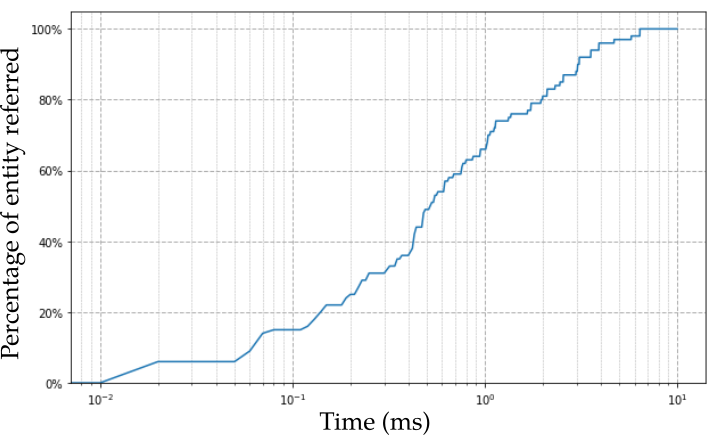
\includegraphics[scale=0.55]{figures/chapter4/scaling_up_percentage.png}
\caption{\label{fig:chap4_percentage} Percentage of entities referred successfully over time using a logarithmic timescale. }
\end{figure}

During a human-robot interaction, a too-long execution time to generate a reference to an entity could spoil the interaction. To assess it we measure the resolution time\footnote{Times reported are run on a CPU Intel Core i7-7700 CPU @ 3.60GHz with 32 Go RAM} of the 77 objects. These measures are reported on the graphic\footnote{The results differ from the original paper because here we are using the latest version of each software to be comparable with the other chapters.} of Figure~\ref{fig:chap4_percentage} and on the table~\ref{tab:reg_solution} in appendix. All the 77 entities (100\%) have been referred in under 6.40ms. This is well below 100ms which is the maximum system response time for the user to get a feeling of instantaneity \cite{miller_1968_response}. Moreover, 50\% are referred under 516\us and 75\% under 1.32ms. On average, the algorithm needs to explore 10.6 nodes to refer to an object. It gives an exploration time of 101.88\us/node on average. All the results over the 77 entities are available on appendix~\ref{app:reg_solutions}.

Regarding the complexity of the solutions, we found that 32 (41.56\%) need at least two relations to be referred to. As the type count for a relation, this means the second relation is one of the entity attributes. Among the others, 25 entities (32.46\%) are referred to through the use of four or more relations. The maximum was six relations for only one of the objects. Moreover, 49.4\% need a reference to another entity in their solution and two objects need references to two others entity in their \acrshort{re}. This mean that 49.4\% of the objects of our situation can not be referred using approaches like \cite{ros_2010_which} or \cite{dale_1995_computational}.

These results over a larger knowledge base highlight the need for a \acrshort{reg} algorithm to use relations and references to other entities to be able to generate suitable \acrshort{re}. They also show the importance of the entities type that is often sufficient with only one attribute to generate an optimal \acrshort{re}. Finally, we demonstrate over these results that our algorithm is suitable for use in human-robot interaction, even with a ``large scale'' knowledge base. With such results, we can even think that it is suitable to be integrated into a planning process needing to request it at high frequency. Such application will be presented in the next chapter.

%count    77.000000
%mean      1.080750
%std       1.355236
%min       0.013237
%25%       0.193782
%50%       0.516371
%75%       1.322064
%max       6.405807

\subsection{Comparisons with other state-of-the art algorithms}

The previous situation has been designed by us and could be adapted for our algorithm. Moreover, existing methods could be more efficient than our. To compare with other algorithms, we choose to perform two comparisons with state-of-the-art algorithms on their domains. Because we saw the importance for a \acrshort{reg} algorithm to be able to refer to entities through relations to other entities and thus through references to other entities, we have only selected methods having this ability.

\subsubsection{The longest-first}

The Longest First (LF)\footnote{\url{http://www.m-mitchell.com/code}} algorithm \cite{viethen_2013_graphs} is a graph based algorithm and it has been tested on the GRE3D3 Corpus. It is composed of 20 scenes. As illustrated if Figure~\ref{fig:chap4_gred3} with the eleventh scene, each is composed of three objects with different spatial relations relative to one another (isOn, isAtLeftOf). Each object have three attributes being a color, a size (small or large) and a type (ball or cube). The entity to refer to is marked by an arrow. This entity has always a direct adjacency relation (e.g. the ball is on the red cube).

Analysing the corpus, we find that 8 target entities can be referenced using only their type (e.g. the ball). Seven entities can be optimally referred to with the use of their type and an attribute (their size or color). In the last five scenes, the target entity can be referred with their types, color and size attributes (e.g. the small green cube). This means that spatial relations have not to be used to reference the target entity. 

\begin{figure}[h!]
\centering
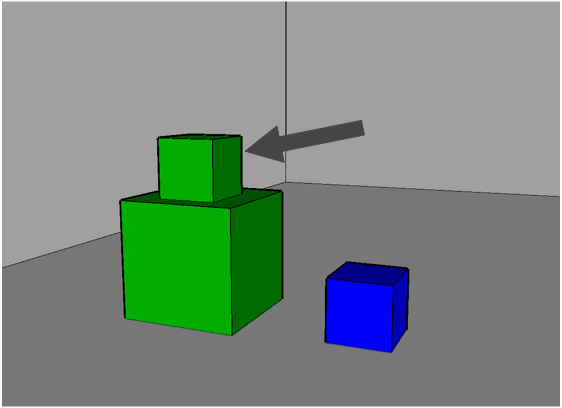
\includegraphics[scale=0.3]{figures/chapter4/GRED3.jpg}
\caption{\label{fig:chap4_gred3} The 19\textsuperscript{th} scene of the GRED3 corpus~\cite{dale_2009_referring}. The target entity is the one marked by the arrow.}
\end{figure}

To perform our analysis, we choose only one of the scene among the ones needing the most attributes. This scene is the 19\textsuperscript{th} of the corpus, illustrated on Figure~\ref{fig:chap4_gred3}. Because the LF does not consider the types\footnote{The objects type are only added as a post-process. This can explain why they use the spatial relations while it is not necessary.}, the chosen scene is only composed of cubes to give comparable solutions. Even if we do not compare with the simple cases, we can note that our algorithm resolves the scene requiring only the type in less than 100\us and those with the types and one attribute in less than 250\us.

The LF algorithm has for objective to generate over-specified REs. To limit the solution length, a maximum length parameter is available on the queries. Setting it to the recommended value, that is 4, we get in 311ms the result which we can read as \textit{``The small green cube on top of a cube''}. Setting it to 3, which is the optimal value for this scene, we get in 109ms the result \textit{``The small green cube''}. This optimal solution is the one found by our algorithm in 0.87ms. The difference factor is thus 125.

For all the 20 scenes, setting the maximum length parameter to the optimal length (the minimum of relations allowing the hearer to distinguish the referred entity without ambiguity), both the LF and our algorithm find the same solutions. However, this parameter raises an issue. In the previous situation of the three-room apartment, 13\% of the entity need more than 4 relations to be referred to. This means that with the recommended value, all these entities would not be referred to while it is possible. On the other hand, we saw that this parameter has a huge impact on the execution time and set it to a higher value would thus require more computational time and give too complex \acrshort{re}.

\subsubsection{The optimized Graph Based Algorithm}

The \acrshort{gba}~\cite{viethen_2013_graphs} has been a significant turning point in the \acrshort{reg} field. We thus compare our algorithm with its more recent optimized version presented in~\cite{li_2017_automatically}. From an entities relations graph dedicated to the task, it aims at finding the lowest cost isomorphic subgraph containing the target entity. To do so, the \acrshort{gba} approach is based on a branch and bound algorithm. Once a first solution is found, any other branch that exceeds the cost of the current best-found solution is bounded. Such an algorithm thus needs to explore a large part of the graph if the optimal solution is not found early in the search.

\begin{figure}[h!]
\centering
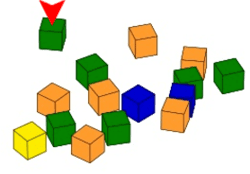
\includegraphics[scale=0.7]{figures/chapter4/GBA.png}
\caption{\label{fig:chap4_gba} The 4\textsuperscript{th} scene used in the user-study in~\cite{li_2016_spatial}. The target entity is the one marked by the red arrow.}
\end{figure}

Their algorithm has been tested on a corpus with 28 tabletop scenes~\cite{li_2016_spatial} as the one presented in Figure~\ref{fig:chap4_gba}. Each scene is composed of 15 cubes of different colors linked through spatial relations and only one of these cubes has to be referred to. To compare our algorithm on their corpus, we selected only one scene (the fourth represented in Figure~\ref{fig:chap4_gba}) and we have converted their graph into an ontology. On this unique scene, we have tested \acrshort{re} generation for each of the 15 cubes composing it. The \acrshort{gba} as well as our algorithm have found a solution for 10 cubes. Because the same costs on relations have been used, both algorithms have found the same solutions. The only difference is that our algorithm has added the objects types. In these 10 cases, our algorithm has performed faster with a factor of 29.4 on average. Because of their use of a branch and bound algorithm, the speed increase is more important for cases with many solutions. We go from a speed factor of 4 for 50\% of the cases, growing to 50 for 25\% of the cases, and reaching 130 at the maximum. For the other 5 cases where no solution is found, both algorithms detect the absence of a solution in a few milliseconds.

The difference with the \acrshort{gba} is that the uniform cost search algorithm ensures the first found solution to be the optimal one. Moreover, because their approach does not use the entities types, we think that our approach should work even faster on knowledge bases containing entities with different types since we prioritize the use of the type. Such a test has not been performed as their algorithm can not manage other data than their corpus.

\section[Integration on a robotic system]{Proof of concept integration on a robotic system}

To assess the usability of our method during an interaction, we have integrated it on a PR2 robotic platform and used it in a ``real'' tabletop scenario. The used architecture presented in this section is represented in Figure~\ref{fig:chap4_archi}.

\begin{figure}[h!]
\centering
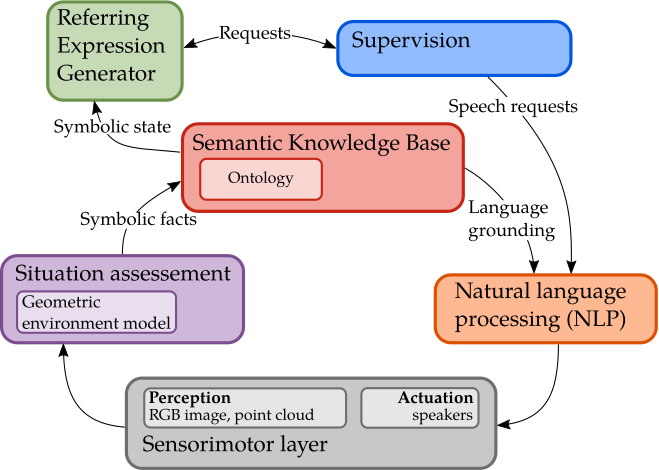
\includegraphics[scale=0.6]{figures/chapter4/architecture.png}
\caption{\label{fig:chap4_archi} The architecture used to validate the method. The knowledge base is continuously kept up to date through the situation assessment.}
\end{figure}

The geometrical situation assessment is based on the Robosherlock~\cite{beetz_2015_robosherlock} perception system. This software does not require any a priori on the environment such as CAD model, mesh or training. With the used pipeline, it detects objects on a surface and gives information about their position, shape (``circular'' or ``rectangular''), color, and size (``large'', ``medium'' or ``small''). On top of that, we have applied simple filtering and tracking based on the previous information. This information is then continuously added to the ontology to kept it up to date with the current state of the environment. Because the objects' types are not determined by the system, all the detected objects are thus added as inheriting from the ``Object'' class. To go further, we could use the SPARK/TOASTER~\cite{milliez_2014_framework} framework to extract higher-level relationships such as ``isOnTopOf'' or ``isIn''. However, the limited information provided by Robosherlock, with the used pipeline, are already interesting to test our algorithm as the robot is not able to use high-level concepts and resulting in various ambiguities.

The knowledge base as an ontology is managed using the software Ontologenius \cite{sarthou_2019_ontologenius}. It is used as a server sharing knowledge about the environment with the entire architecture. Because no perspective-taking is performed, it manages a single instance representing the robot's knowledge. The \acrshort{reg} is thus performed on this instance even if it should rather be run on the human partner's estimated knowledge.

\begin{figure}[b!]
\centering
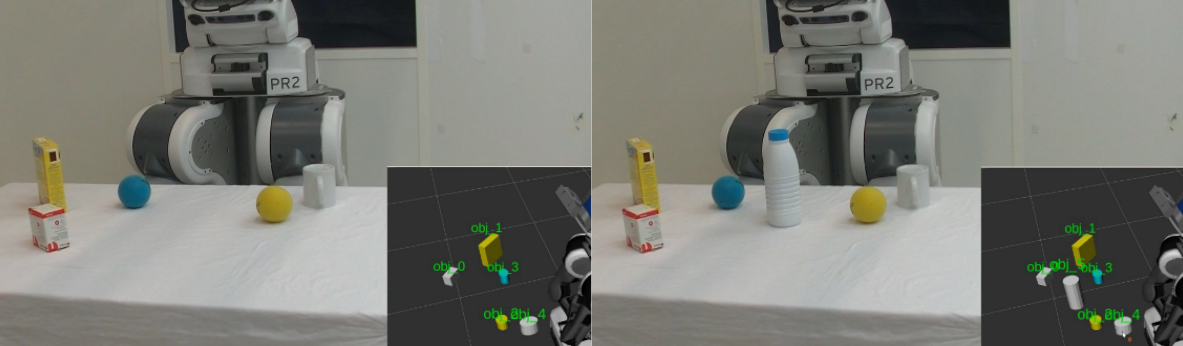
\includegraphics[width=\textwidth]{figures/chapter4/pr2.png}
\caption{\label{fig:chap4_pr2} Two situations where the robot has to refer to the cup on the right of the image. The presence of the milk bottle (with the red circle on the image on the right and the red arrow in the RVIZ view) changes the generated \acrshort{re}. On the right-bottom part of each image is displayed the geometrical representation of the scene as perceived by the robot.}
\end{figure}

An ad hoc linguistic realisation has been made, based on simple grammar and the labels present in the ontology. It takes as input a \sparql{} query and is able to generate a sentence in English or in French depending on the ontology configuration. For example, it is able to transform the query ``?0 isA Cup, ?0 isOn ?1, ?1 isA Table, ?1 hasColor black'' into ``\textit{the cup on the black table}''. The relations in the query do not have to be ordered as the link between the variable can be analysed and a simple language model provides the attribute order for each language.

The scenario \footnote{Commented video available at: \url{https://youtu.be/mKDLvDbHfvkit }} consists of several objects on a table. As illustrated on the left part of Figure~\ref{fig:chap4_pr2}, the initial situation is composed of five objects. The robot has to generate a \acrshort{re} for the cup. The found solution can be verbalized as\textit{``The white circular object''} since there are other non-white circular objects and other white non-circular objects. In a second time, a human adds a milk bottle on the table (right part of Figure~\ref{fig:chap4_pr2}). Because the bottle is circular and white, the previous \acrshort{re} is no more valid. When the robot is asked to describe the cup, it generates this time the sentence \textit{``The white small circular object''}. The addition of the size attribute solve the introduced ambiguity.

With this simple task, we show that our \acrshort{ucs} ontology-based \acrshort{reg} algorithm is usable within a robotic architecture, can deal with a dynamic environment, and can adapt its explanation to the current situation.
